%% ----------------------------------------------------------------
%% Project Report - Adam Mulligan
%%
%% Template based on http://www.sunilpatel.co.uk/thesis-template/
%% ---------------------------------------------------------------- 

\documentclass[a4paper, 11pt, oneside]{Thesis}  % Use the "Thesis" style, based on the ECS Thesis style by Steve Gunn
\graphicspath{{Figures/}}  % Location of the graphics files (set up for graphics to be in PDF format)

\usepackage[square, numbers, comma, sort&compress]{natbib}  % Use the "Natbib" style for the references in the Bibliography
\usepackage{verbatim}  % Needed for the "comment" environment to make LaTeX comments
\usepackage{vector}  % Allows "\bvec{}" and "\buvec{}" for "blackboard" style bold vectors in maths
\hypersetup{urlcolor=black, colorlinks=false}

%% =====================
% SETUP & TITLE PAGE

\begin{document}
\frontmatter

\title  {Enigma: Prime Numbers and Cryptosystems}
\authors  {\texorpdfstring
            {\href{http://cyanoryx.com}{Adam Mulligan}}
            {Adam Mulligan}
            }
\addresses  {\groupname\\\deptname\\\univname} 
\date       {\today}
\subject    {}
\keywords   {}

\maketitle

%% =====================
% STYLES

\setstretch{1.3}  

\fancyhead{}  
\rhead{\thepage}  
\lhead{}  

\pagestyle{fancy}  


%% =====================
% QUOTE

\pagestyle{empty} 

\null\vfill
\textit{``Anyone can design a security system that he cannot break. So when someone announces, “Here’s my security system, and I can’t break it,” your first reaction should be, “Who are you?” If he’s someone who has broken dozens of similar systems, his system is worth looking at. If he’s never broken anything, the chance is zero that it will be any good.''}

\begin{flushright}
Bruce Schneier, \textit{The Ethics of Vulnerability Research}
\end{flushright}

\vfill\vfill\vfill\vfill\vfill\vfill\null
\clearpage 

%% =====================
% ABSTRACT

\addtotoc{Abstract} 

\abstract{
	\addtocontents{toc}{\vspace{1em}}  % Add a gap in the Contents, for aesthetics

	Modern cryptography allows us to perform many types of information exchange over insecure 
	channels. One of these tasks is to agree on a secret key over a channel where messages can 
	be overheard. This is achieved by Diffe-Hellman protocol. Other tasks include public key 
	and digital signature schemes; RSA key exchange can be used for them. These protocols are 
	of great importance for bank networks.

	Most such algorithms are based upon number theory, namely, the intractability of certain 
	problems involving prime numbers. The project involves implementing basic routines for 
	dealing with prime numbers and then building cryptographic applications using them.
}

\clearpage 

%% =====================
% ACKNOWLEDGMENTS

\setstretch{1.3}  % Reset the line-spacing to 1.3 for body text (if it has changed)

% The Acknowledgements page, for thanking everyone
\acknowledgements{
\addtocontents{toc}{\vspace{1em}}  % Add a gap in the Contents, for aesthetics

With thanks to my project advisor Yuri Kalnishkan, and the RHUL Department of Computer Science for three years worth of knowledge and experience.

}
\clearpage  % End of the Acknowledgements

%% =====================

\pagestyle{fancy} 

%% =====================

\lhead{\emph{Contents}}  
\tableofcontents  % Write out the Table of Contents

%% =====================

\lhead{\emph{List of Figures}} 
\listoffigures  % Write out the List of Figures

%% =====================

\lhead{\emph{List of Tables}}  
\listoftables  % Write out the List of Tables

%% =====================
% ABBREVIATIONS

\setstretch{1.5}  
\clearpage  

\lhead{\emph{Abbreviations}}  

\listofsymbols{ll}  {
	\textbf{AES} & \textbf{A}dvanced \textbf{E}ncryption \textbf{S}tandard \\
}

%% =====================
% CHAPTERS

\mainmatter
\pagestyle{fancy}  

\chapter{Introduction}
\label{Chapter1}
\lhead{Chapter 1. \emph{Introduction}}

\section{What it is about}

Secrecy has always been of great importance, not just in modern society, but throughout history. Until very recently, Cryptography was consigned to the sending and receiving of messages, generally using pen and paper. However, increasingly cryptography -- the study and implementation of techniques for secure communication -- is becoming more vital to the smooth running of even basic systems, whether it is the clich\'{e} example of military secrets or simply a micro-payment for an online service. Initially, the usage of provably secure and efficient cryptographic algorithms was limited to governments and related contractors, however the advent of cryptographic standards, and more relevantly the creation of public-key cryptography mechanisms, has pushed it in to a wider field of use as researchers gained a better understanding of the area. 

\section{Goals and Intentions}

The primary goal of this project can be found in the title and abstract: to research, discuss and create algorithms within or related to the field of prime numbers. To complete this task I will be developing my thoughts and discoveries regarding prime numbers as this report progresses, as well as producing a number of deliverables in the form of software applications, test results and statistics.The topic of number theory is in itself fascinating, and extraordinarily vast, however I will only be scratching the surface. Nonetheless, I hope to explain throughout this project how prime numbers have become such an important part of modern cryptography, and what they can be used for.

\section{Project Summary}

I will be splitting the project in to three main parts, excluding this report:

\begin{enumerate}
	\item \textbf{Prime numbers in software} \\
		A discussion of how prime numbers can be efficiently produced programmatically, and the software to prove it.
	\item \textbf{Algorithms} \\
		The development of algorithms using prime numbers, such as RSA, and complementary cryptographic algorithms such as AES. Alongside this, the development of non-major algorithms in the field of prime number based cryptography that still present academically interesting concepts.
	\item \textbf{Final Application} \\
		The production of a software program that utilises the implemented cryptographic algorithms in \textsection\ref{Chapter2} to display their efficacy in a real world application.
\end{enumerate}

The primary algorithms to develop are:

\begin{itemize}
	\item Asymmetric
		\begin{itemize}
			\item RSA
			\item Diffie-Hellman
		\end{itemize}
	\item Symmetric
		\begin{itemize}
			\item AES
		\end{itemize}
	\item Identification and Authentication
		\begin{itemize}
			\item RSA Signing
			\item Digital Certificates
		\end{itemize}
\end{itemize}

The reasoning behind this selection is thus: popularity. The best algorithms are those that are mature and have been scrutinised thoroughly by an open source community. However, we will further discuss this choice as the report progresses. Other algorithms will be discussed and produced alongside these, however they will not be used in the final application testbed and are purely for research interest. These can be found listed in the contents in the relevant sections.
		
\section{Other Information}

This document was written and composed with \LaTeX \ using \emph{Taco Software's} Latexian\footnote{http://tacosw.com/latexian/}. The \LaTeX \ source code for this report should have come bundled with the project documentation and files, however if you are unable to retrieve it please see \emph{\textsection \ref{sec:project_repo}}.

\emph{Eclipse Indigo}\footnote{http://eclipse.org} was used for Java development, the primary language used in this project, along with \emph{MacVim}\footnote{http://code.google.com/p/macvim/} for general source and text editing.

Git with \emph{GitHub}\footnote{http://github.com} was used for source control, with \emph{GitHub Issues} used for bug tracking. \emph{Trello}\footnote{http://trello.com} was used for idea and to-do management. \emph{OmniGraffle}\footnote{http://www.omnigroup.com/products/omnigraffle/} was used to produce graphics, such as sequence diagrams and system overviews.

\subsection{A note on openness}

As with any field of study, the quality of research and development is dependent on the open distribution and sharing of ideas. This is \emph{particularly} important with regards to cryptography. As said, cryptography was once reserved to government and research was conducted in secrecy. The open sharing of relevant information in this field is not just for the furthering of knowledge, but also to allow others to inspect and examine algorithms, a process that drastically improves the security of a system. As such, the entirety of this project is licensed under the \textbf{GNU Lesser General Public License version 3 or greater} and is available for access publicly online.

\subsection{Project Repository}
\label{sec:project_repo}

\textbf{If any part of this report is missing, you believe that you do not have a full access to the source code discussed in this document, or if any files have been lost, it is available for full download at \url{http://cyanoryx.com/files/project.tgz}}. 

% Chapter 2

\chapter{Cryptographic Primitives} % Write in your own chapter title
\label{Chapter2}
\lhead{Chapter 2. \emph{Cryptographic Primitives}} % Write in your own chapter title to set the page header

\section{Basics of Information Security}

Despite how it is portrayed or colloquially used, Information Security is an entirely different concept and area of study compared to Cryptography. It might seem simple enough to implement a basic cryptographic protocol involving encryption and decryption, however to introduce this into a system and expect the information to be secure, is foolhardy. Cryptography is a \emph{means} to providing information security when following certain rules and guidelines not the be all, end all solution. An understanding of information security, and the related issues, is necessary. 

This can be proven using historical evidence: throughout history many complex systems of mechanisms, rules, and protocols have been developed to introduce information security to a system. As with modern day security, this cannot be achieved entirely through mathematical and cryptographic means -- it is more than just computational intractability.

As such, stringent criteria for developing secure systems and protocol have been introduced. While institutes such as \emph{The British Computing Society} and \emph{Association for Computing Machinery} ensure their members follow a professional code of ethics, just as a doctor might, these information security criteria are of separate and equal importance. Indeed, there are now several international organisations that exist solely for the overseeing of cryptographic research and development (See: \emph{International Association for Cryptologic Research}).

Often, as we will see, cryptographic systems are simplified for the purposes of presentation particularly for textbooks. This will be discussed further later, with regards to the differences and difficulties involved in developing systems that do not just follow a mathematical "recipe," but also include information security values and other subtleties.

The overall method of dealing with, and ensuring, information security is known as risk management. This encapsulates a large number of countermeasures (including cryptography) that reduce the risk of vulnerabilities in, and threats to, systems. We will only be encountering and discussing the technological areas of mitigation, however some of the solutions include\footnote{For an excellent resource regarding information security, both technical and non-technical, see \href{http://www.cl.cam.ac.uk/~rja14/book.html}{\emph{Security Engineering}, Ross Anderson}}: access control, security policy, physical security, and asset management.

\section{Objectives}

As said, secure systems should follow a guideline, or set of criteria, that ensure the security and integrity of data stored and input. A clear and concise specification should be developed, that will aid the designer in selecting the correct cryptographic primitives, but also help the engineer implement the protocol correctly. There are many of these criteria, however each is derived from four primary objectives:

\begin{enumerate}
	\item \textbf{Confidentiality} is the ability to ensure data is only accessed by those who are allowed to. Maintaining confidentiality of data is an obligation to protect someone else's secret information if you have been entrusted with it.
	\item \textbf{Authentication} involves identifying both entities and data. Two or more entities wishing to communicate or transmit information to one another must identify each participant to ensure they are who they claim to be - this is known as entity authentication. Data received must be authenticated to ensure the validity of the origin, date sent, contents, etc - this is known as data origin authentication.
	\item \textbf{Non-repudiation} prevents an entity from denying previous actions they have committed.
	\item \textbf{Data Integrity} is how faithfully data compares to it's true state, i.e. proving that a data object has not been altered.
\end{enumerate}

\section{Key Concepts}

As with any discipline, there are a number of fundamental concepts that need to be thoroughly defined. This section will cover the definitions of basic information security and cryptography related concepts. While Computer Scientists and Mathematicians, unlike Biologists, tend to abstract ideas using existing words such as \emph{normal} which ultimately cause confusion to those trying to understand the area of study, the field of Information Security fortunately uses phrases that are succinct and aptly describe notions.

\textcolor{red}{TODO: er, do this bit.}

\section{Primitives}

As we discussed in the Objectives, there are certain criteria that must be met for an application to be considered as secure under Information Security guidelines. Excluding physical and psychological measures, there are a number of methods to be implemented cryptographically to guarantee security.

\subsection{Encryption}

Being what is seen as the very 'core' of cryptography, we have defined encryption many times already and what the term means in terms of a process should be apparent. However encryption takes many forms, with each having an appropriate situation for it to be used.

\subsubsection{Symmetric Key Encryption}

Primarily, we will use symmetric key encryption algorithms to encipher data that is to be transmitted between entities.

Mathematically we can formally define symmetric encryption as:

For a message $M$, algorithm $A$ and key $K$,

$M'  = A(K,M)$

and thus:

$M = A'(K',A(K,M))$

where $A' = A$, $K' = K$ in a symmetric algorithm.

\subsection{Key Agreement}

Key agreement, or key exchange, primarily ensures data integrity and confidentiality. By preventing an attacker from discovering encryption keys used on transmitted data, the attacker should be unable to feasibly read confidential information or modify it (the latter is not entirely true, it may be possible in some cases to modify encrypted data, however we will discuss that later in \emph{Symmetric Cryptography}).

While it might be easier to use asymmetric techniques to encrypt data for transmission, thus allowing us to distribute keys as cleartext, it is slow and inefficient for large quantities of data, such as in an instant messaging application. Because of this, it is prudent to implement an efficient symmetric key encryption algorithm, and share the key (known as a session key) with other entities. However, it would be trivial for an attacker to launch a man-in-the-middle attack and gain access to the encryption keys during the initiation of the conversation, allowing the easy and undetectable decryption of all transmitted messages. As such, session keys will need to be distributed using a key exchange protocol.

\subsubsection{Key Distribution Centre}

The simplest solution is known as a Key Distribution Centre (KDC), which involves the use of a trusted third party (TTP). It is easiest to explain using an example. Alice and Bob are users of a system, attempting to securely communicate. Each share a key securely with third-party Trent (somewhat amusingly, this algorithm does not include how these keys should be shared. We can assume that it was perhaps conducted through an in-person meeting of entities, or other means), who stores each key. 

\begin{enumerate}
	\item Alice initiates a conversation with Bob.
	\item Alice requests a session key from Trent, who makes two copies of an identical key and encrypts one with Alice's stored key, and another with Bob's.
	\item Alice receives both encrypted keys, and sends the appropriate one to Bob.
	\item Alice and Bob decrypt their session keys, leaving both with a shared key.
	\item Alice and Bob can now encrypt and decrypt data using the same key.
\end{enumerate}

\subsubsection{Asymmetric Cryptography}

As can be obviously seen, using a KDC is dependent entirely on the ability of two entities to have previously, and securely, shared an encryption key with a TTP that is known to both entities. A solution to this is to eliminate the third party, and use an asymmetric algorithm to share keys directly. As defined in the \emph{Key Concepts} section, asymmetric cryptography allows Alice to share a public-key, with which any entity can encrypt data that can only be decrypted using Alice's private key.

\begin{enumerate}
	\item Alice and Bob share their public keys using a readily available database.
	\item Alice downloads Bob's key, and vice versa.
	\item Alice generates a session key, encrypts it using Bob's public key and sends it to Bob.
	\item Bob can now decrypt the session key using his private key, resulting in both parties being in possession of a secure session key.
\end{enumerate}

There is a security risk: how can you verify that the entity that sent the encrypted key is indeed the one with which you are trying to communicate? It would be easy for an attacker to encrypt their own session key with Alice's public key, and claim that the key is from Bob. The attacker would then be able to decrypt any messages intended for Bob. The solution to this issue is the use of digital certificates, and signatures, which will be discussed in \emph{Authentication}.

We will discuss specific algorithms further on, however it is worth pointing out that the current public-key algorithms used for these purposes are \emph{RSA} (Rivest, Shamir, Adleman) and the \emph{Diffie--Hellman Key Exchange Protocol}. There exist a number of interesting algorithms that implement the public key architecture which will also be considered later.

There are other considerations in key management to ensure confidentiality and integrity. Some provisos exist such as changing the key for each session to ensure perfect forward secrecy, however these are trivial to implement and can be considered as part of the overall application security development.

\subsection{Authentication}

There are two types of authentication that are required in a secure application

\begin{enumerate}
	\item Message authentication
	\item Entity authentication
\end{enumerate}

both of which require different protocols and algorithms. These terms have been defined in \emph{Objectives}.

The methods of entity authentication are an interesting topic in themselves, with many, many protocols having been researched and created as the community tries to find a method that is both secure and easy for an entity to use. Some examples are: passwords, two-factor authentication, PINs, smart cards, biometrics, and so on. These are outside of the scope of this project -- we will be implementing two broad, yet specific methods of authentication.

\subsection{Digital Signatures}

Digital signatures, as we will see, encompass three of the information security criteria: authentication, data integrity and non-repudiation (a sender cannot claim they did not send the message). A digital signature is a string that connects a message with its originating entity.

When transmitting a message, the sender signs the message with their private key which can then be verified with their public key, which should be available to the receiver.

\begin{enumerate}
	\item Alice signs her message $A$ with her private key.
	\item Alice sends message $A$ with signature $S$ to Bob ($A|S$)
	\item Bob retrieves Alice's public key from an available database, and verifies signature $S$
\end{enumerate}

The first and most common implementation of digital signatures is RSA.

\subsection{Public-key Certificates}

Digital signatures and a public-key infrastructure, however, are not enough by themselves. A very simple attack can be orchestrated similar to that during key agreement: Mallory, the attacker, could sign a modified message $A$ with her own private-key and then distribute her public-key, claiming it to be Alice's. To counter this, we can introduce a trusted third-party, known as a Certificate Authority (CA), who signs Alice's public-key with their own private-key. Most trusted CA's public keys come bundled with software such as browsers and operating systems.

\begin{enumerate}
	\item Certificate Authority signs Alice's public key with their private key.
	\item The CA distributes its public key with major software.
	\item Bob receives Alice's message and signature, as well as her public key and signature.
	\item Bob verifies Alice's public key with the CA's public key, and then verifies the message.
\end{enumerate}

\subsection{Hashing}

While not of direct relevance in information security, hashing plays a significant part in cryptographic systems and thus is included as a concept to be implemented. Formally, we can define a hash function as mapping a large domain to a smaller range - in the case of data, mapping a set of bytes to a unique identifier with a set length. A hash function, at the very basics, takes as input a message and produces a fingerprint, or digest, of the input. Within the field of cryptography, they are used for message authentication and data integrity.

This is to say, given a domain $D$ and range $R$ for $f : D \rightarrow R, then |D| > |R|$. This is a many-to-one relationship, the downside of which means that collisions can occur -- two input strings resulting with the same output string -- however, this varies between algorithms, the more modern of which are less likely to result in collisions.

A hash function can be classed into two categories: keyed and unkeyed, taking both a message and secret key and taking just a message, respectively. Two conditions are necessary for a hash function to be effective:

\begin{enumerate}
	\item compression -- the function $f$ maps input $a$ of arbitrary length to an output of fixed length, $n$.
	\item complexity -- it must be easy to compute $f(a)$
\end{enumerate}

Most commonly used are unkeyed, one-way hash functions. Some examples of which are: SHA-1, and MD5. In cryptography, hashes are commonly used for data integrity in combination with digital signatures. A message is hashed, and the fingerprint produced is signed by the entity. There are some algorithms designed specifically for this purpose, known generally as Message Authentication Codes (MACs) and Manipulation Detection Codes (MDCs).

A sample of each of these four primitives will be implemented further in the report.

\section{Mathematics}
\newtheorem{mathdef}{Definition}[section]
\newtheorem{mathexample}{Example}[section]
\newtheorem{mathfact}{Fact}[section]

This section will cover some of the basic mathematical concepts that will be used throughout the report, and form a foundation of understanding for the more complex abstract methods that will be used.

\subsection{Notation}

\begin{enumerate}
	\item $\mathbb{Z}$ is the set of all integers.
	\item $\mathbb{R}$ is the set of all real numbers.
	\item $[a,b]$ is the set of integers $n$ such that $a\le n \le b$.
	\item $|A|$ is the cardinality of a finite set, i.e. the number of elements.
	\item $n \in A$ denotes that an element $n$ exists in set $A$.
	\item $A \subseteq B$ denotes that set $A$ is a subset of set $B$.
	\item $A \subset B$ denotes that $A$ is a subset of $B$, but $A \neq B$.
	\item $\lceil a \rceil$ is the smallest integer greater than or equal to $a$.
	\item $\lfloor a \rfloor$ is the largest integer less than or equal to $a$.
	\item A function (mapping) denoted as $f : A \rightarrow B$ signifies that every element $a$ in $A$ is mapped to exactly one element $b$ in $B$. This can also be written as $f(a) = b$.
\end{enumerate}

\subsection{Number Theory}

We will begin by defining some fundamental rules of number theory. 

\begin{mathdef}
	Let $a,b$ be integers. $a$ divides $b$ if an integer $c$ exists such that $b = ac$. We define this as $a$ divides $b$, or $a|b$.
\end{mathdef}

\begin{mathdef}
	An integer $c$ is a common divisor if $c|a$ and $c|b$.
\end{mathdef}

\begin{mathdef}
	An integer $c$ is the greatest common divisor of $a$ and $b$, if:
	\begin{enumerate}
		\item $c$ is a common divisor of $a,b$.
		\item when $d|a$ and $d|b$, $d|c$.
		\item $c\ge0$
	\end{enumerate}
	This is denoted as $c = $ gcd$(a,b)$.
\end{mathdef}

\begin{mathdef}
	An integer $a$ is prime if:
	\begin{enumerate}
		\item $a\ge2$
		\item the only positive divisors are $1$ and $a$.
	\end{enumerate}
	Otherwise, the number is referred to as composite.
\end{mathdef}

\begin{mathfact}
	There are an infinite number of prime numbers.
\end{mathfact}

\begin{mathdef}
	If $a$ is prime and $a|bc$, then $a|b$ and $a|c$.
\end{mathdef}

\begin{mathdef}
	Integers $a$ and $b$ are relatively prime (coprime) to one another, if gcd$(a,b)=1$.
\end{mathdef}

\begin{mathdef}
	The function $\phi$ is known as the Euler Phi function. Where $n\ge1$, $\phi(n)$ is the number of integers in the interval $[1,n]$ that are relatively prime to $n$.
	\begin{enumerate}
		\item If $n$ is prime, then $\phi(n) = n - 1$.
		\item $\phi(n)$ is multiplicative: if gcd$(m,n) = 1$, then $\phi(mn) = \phi(m) \cdot  \phi(n)$.
	\end{enumerate}
\end{mathdef}

\subsubsection{Modulo Arithmetic}

\begin{mathdef}
	Where $a$ and $b$ are integers, $a$ is congruent to $b$ modulo $n$ (denoted as $a \equiv b  \mod n$. $n$ is known as the modulus. Congruence is reflexive, transitive and and symmetric. That is to say, for every $a,b,c \in \mathbb{Z}$:
	\begin{enumerate}
		\item $a \equiv a  \mod n$
		\item if $a \equiv b  \mod n$, then $b \equiv a  \mod n$
		\item if $a \equiv b  \mod n$ and $b \equiv c  \mod n$, then $a \equiv c  \mod n$
	\end{enumerate}
	This is known as an equivalence relation.
\end{mathdef}

\begin{mathdef}
	The set of all integers modulo $n$ is denoted as $\mathbb{Z}_n$.
\end{mathdef}

As you can see, there are a great number of theorems regarding prime numbers and modulo arithmetic (we have barely scratched the surface), some of which we will be using.

\subsection{Abstract Algebra}

Further on, particularly in the development of symmetric algorithms like AES, we will be using groups, fields and other abstract algebraic objects. Due to the complex nature of these concepts, they will be explained in tandem with the algorithms themselves.

\subsection{Complexity}

Computational complexity is a vast subject, mostly out of the scope of this report, however we will use the notation occasionally to classify algorithms. Big-oh notation, as it is known, will be used to represent the worst-case running time of an algorithm based on a standard input size. For example:

\begin{mathdef}
	A polynomial-time algorithm is an algorithm where the worst-case running time can be represented as $O(n^c)$, where $n$ is the input size, and $c$ is a constant. 
\end{mathdef}

An algorithm with a running time that cannot be bounded as such is known as an exponential-time algorithm. It is generally considered that polynomially-time algorithms are efficient, wheres exponential-time algorithms are inefficient.

\section{Moving On}

This is just a basic overview of the cryptographic and mathematical primitives used in Information Security. As the report progresses, each concept will be explained in finer detail alongside their implementations. While it seems hard to apply these abstract definitions, the purpose of each within our algorithms will become quickly clear. 

% Chapter 3

\chapter{Number Theory and Public-key Cryptography}
\label{Chapter3}
\lhead{Chapter 3. \emph{Number Theory and Public-key Cryptography}} 

\section{Overview}

Number theory, the unit of mathematics that studies integers and their properties, was once a predominantly useless area. However, as cryptographic algorithms became more prevalent, particularly schemes that require the use of large prime numbers. We have already covered the notation used in the majority of number theoretic algorithms, and so this section will build upon this and discuss basic concepts and applications: modular arithmetic, prime number generation, and factorisation.

In this section we will make the assumption that any attackers who may try to break our algorithms or eavesdrop on our messages are extremely powerful and capable, and so we will discuss algorithms with regards to their tractability -- in this case, whether or not a significant percentage of all instances of a problem can be solved in polynomial time.

Throughout, where appropriate, programming examples are provided in Java.

\section{Modular Arithmetic and Congruence}

  As we know, the core concept of modular arithmetic is to return the remainder of the division of two integers, represented as $a(mod \ n)$. It is said that $b$ is congruent to $a(mod \ n)$ if $b \equiv a(mod \ n)$. Congruences play a great part in cryptography -- one of the very first uses was the Caesar Cipher. Messages were made secret -- encrypted -- by shifting letters forward by an integer $n$, where $0 < n \leq 25$.
  
  Given a sequence of characters $\{A,B,C,...,Z\}$ where each letter is represented by a number $\{0,1,2,...,25\}$. Defined by a function $f(n)$, where $n$ is the integer representation of a character:
  
    \begin{center}
       $f(n) = (n + x) \ mod \ 26$
    \end{center}
    
  where $x$ is the number of characters to shift by.
  
  This is a very simple example of how congruences can be used in cryptography. As we will see in the public-key section, congruences can be applied in a similarly simple way as a vital component part of a far more complex algorithm.
  
  Indeed, although the technicalities of this are not relevant, congruences can even be used to generate pseudo-random numbers.

\section{Prime Numbers}

Primes have already been covered, however they are a deeply fascinating subject with many current open problems and conjectures. For example, Goldbach's Conjecture states that every odd integer $n$, where $n > 2$, is the sum of two primes. This is intriguing because so far this has been \emph{verified} for integers up to $2 \times 10^{17}$, but mathematicians have not yet found a formal proof for this, and despite this they continue to believe it to be true \cite{Rosen:2007aa}.

We, however, will be using them for a far more interesting\footnote{http://xkcd.com/247/} purpose: cryptography based around the intractability of factoring very large composite numbers into their smaller non-trivial prime divisors.

  \subsection{Generation}
  
  First and foremost, we must devise an efficient method for generating the prime numbers. Although generating the keys for use in prime number based algorithms is generally not done on a regular basis, it is still a complex task to complete in a reasonable amount of time. As it stands, a number of algorithms already exist (and have done for many hundreds of years) for this purpose, though in a different sense: it is relatively easy to generate small sequences of small primes, however to obtain large, individual primes the fastest method is to generate probable primes using primality tests.
  
  To help understand these algorithms, we must first state a number of theorems that make clearer how these algorithms work and how they will fit in to the public-key implementations later on \cite{Alfred-Menezes:1996kx}: \\
  
  \begin{mathdef}
    We define $\pi(x)$ as the number of primes found in the interval $[2,x]$, where $\pi(x) \sim \frac{x}{\ln x}$.
  \end{mathdef}
  
  \begin{mathfact}
    If $gcd(a,n) = 1$, there are infinitely many primes that are congruent to $a \mod{n}$.
  \end{mathfact}
  
  \begin{mathfact}
    We can say that all prime numbers are uniformly distributed across $\phi(n)$ because:
    \begin{center}
    	$\pi(x,n,a) \sim \frac{x}{\phi(n) \ln x}$
    \end{center}
    Where $\pi(x,n,a)$ is the number of primes in the interval $[2,x]$ congruent to $a \mod{n}$.
  \end{mathfact}
  
  \begin{mathfact}
    We can approximately determine the $n$th prime number as $\rho_n \sim n \ln n$, where $n \geq 6$.
  \end{mathfact}
  
    \subsubsection{Probable, Provable and Pseudo-primes}
    
    There is a subtle yet significant difference between the types of primes that can be generated.
    
      \paragraph{Probable Primes}
      
      A probably prime is a prime that meets certain conditions that are satisfied by all prime numbers. Testing for probably primes are more appropriately known as \emph{compositeness tests} rather than probable primality tests.
      
      The algorithms we will define as probabilistic primality tests will take arbitrary integers and test them to provide information about their primality. 
      
      \paragraph{Pseudo-primes}
      
      Pseudo-primes are a subset of probably primes. They are composite numbers that pass tests that most composite numbers fail, for example an integer is pseudo-prime if it satisfies Fermat's Little Theorem.
      
      \paragraph{Provable Primes}
      
      A provable prime is a prime that can be formally proven to be prime using an algorithm, such as the AKS primality test. Generally these are not used in cryptography due to the previous inefficiency of calculating provably-prime numbers, and also as they work most effectively when the input has been passed through a probabilistic primality test first.
  
    \subsubsection{Sieves}
    
    A prime sieve is a fast algorithm to find prime numbers, the most commonly used being the \emph{sieve of Erastothenes} and \emph{sieve of Atkin}. Prime sieves operate by generating a list of integers up to a defined limit $n$: $\{2,3,4,...,n\}$ and progressively removing the composite integers in line with particular rules. However, this is very slow for the generation of individual large primes, and so is immediately discounted from possible use in a cryptographic algorithm.
    
    \subsubsection{Fermat's Little Theorem}
    
    \textbf{Note:} Fermat's theorem is no longer considered to be a true probabilistic primality test as it cannot determine the difference between probable primes and composite integers known as Carmichael numbers\footnote{Carmichael numbers are similar to Fermat primes as they satisfy the congruence $b^{n-1} \equiv 1 \mod{n}$. The conditions for a number to be in the Carmichael set are more complex than this, however the details are out of the scope of this section.}. The theorem can still be used to prove the compositeness of a number.
    
    Fermat's theorem states:
    
    \begin{center}
      If $n$ is prime and $a$ is an integer, $1 \leq a \leq n - 1$, then
      $a^{n-1} \equiv 1 \mod{n}$
    \end{center}
    
    Using this, we can take an integer $n$ and to test for primality find an integer in this interval where the equivalence is not valid, thus proving that $n$ is composite, and is not likely to be prime.
    
    The implementation of this in Java is as so:
    
    \lstset{language=Java}
    
    \lstinputlisting{./Code/primes/FermatTesting.java}
    \emph{This file can be found at latex\_src/Code/primes/FermatTesting.java}
    
    This is a very simple algorithm to implement. It selects a random integer in the interval $[1,n-1]$ and computes $a^{n-1}$. If $a \neq 1$, then $a$ must be composite.
    
    \textbf{Note:} We are using the class \verb!BigInteger! to represent integers, as it allows far larger bit representations of integers than Java's standard 64-bit primitive \verb!integer! type. \verb!BigInteger! offers all the same operators that can be used with \verb!integer! primitives, alongside useful operations such as modular arithmetic, GCD and even built in primality testing. We will use \verb!BigInteger! for all Java-based programming that involves large integers.
    
    \subsubsection{Miller--Rabin Primality Test}
    
    In practice, the Miller--Rabin test is the most used primality test, that also is based on a set of equivalences that are true for primes, and thus if a number to be checked does not pass these equivalences it is not prime. \\
    
    \begin{mathdef}
      Let $n$ be an odd prime: $n - 1 = 2^dr$, where $d$ and $r$ are positive integers, with $r$ being odd. For $a \in (\mathbb{Z}/n\mathbb{Z})$: \\
      $a^r \equiv 1 \mod{n}$ \textbf{or} \\
      $a^{2^dr} \equiv -1 \mod{n}$ assuming $0 \leq d \leq s - 1$.
    \end{mathdef}
    
    Using this, we can define the Miller--Rabin requirements as:
    
    \begin{enumerate}
      \item Assume $n$ is an odd composite integer, and $n - 1 = 2^sr$, where $r$ is odd.
      \item Where $a$ is an integer in the interval $[1,n-1]$, if $a$ does not match the conditions in definition 3.3.2 ($a^r \not\equiv1 \mod{n}$,  $a^{2^sr} \not\equiv -1 \mod{n}$), then $a$ is known as a witness for $n$.
      \item Where $a$ is the same as $a$ in point 2, if $a$ matches \emph{either} of the conditions in definition 3.3.2, it is known as a strong liar for $n$.
    \end{enumerate}
    
    When $n$ is determined to be a composite, it is known as a \emph{witness}, meaning it is a definite composite number. When we refer to probable primes, they are known as \emph{strong liars} as they are a likely probably prime to the base integer -- it is known as a "strong" liar due to the fact that $n$ could still be composite while the prime equivalences still hold.
    
    The implementation of this in Java is as so:
    
    \lstinputlisting{./Code/primes/MillerRabinTest.java}
    \emph{This file can be found at latex\_src/Code/primes/FermatTesting.java}
    
    In some cases the number of iterations is known as the \emph{security parameter}.
    
    \subsubsection{Solovay--Strassen Primality Test}
    
    The Solovay--Strassen test was one of the first primality tests to be made popular by the increasing use of public-key cryptography. It is another probabilistic primality test. It is, in essence, quite a simple algorithm in that the process flow is linearly straightforward. \\
    
    \begin{mathdef}
      Let $n$ be an odd integer, then $a^{\frac{(n-1)}{2}} \equiv (\frac{a}{n}) \mod{n}$ where gcd$(a,n) = 1$.
    \end{mathdef}
    
    We can use this to define the Solovay--Strassen algorithm requirements:
    
    \begin{enumerate}
      \item If gcd$(a,n) > 1$ or $a^{\frac{(n-1)}{2}} \not\equiv (\frac{a}{n}) \mod{n}$, then $a$ is an Euler witness for $n$ (composite).
      \item If gcd$(a,n) = 1$ and $a^{\frac{(n-1)}{2}} \equiv (\frac{a}{n}) \mod{n}$ then $n$ is an Euler pseudoprime (prime).
    \end{enumerate}
    
    This is relatively simple to implement:
    
    \lstinputlisting{./Code/primes/SolovayStrassenTest.java}
    \emph{This file can be found at latex\_src/Code/primes/SolovayStrassenTest.java} \\
    
    \begin{mathdef}
      $(\frac{a}{n})$ is known as the Jacobi symbol, and plays an important part in the Solovay--Strassen test. Let $m,n$ be odd integers where $m \geq 3$ and $n \geq 3$, and $a,b \in \mathbb{Z}$, then we have the following properties\cite{Alfred-Menezes:1996kx}:
    
      \begin{enumerate}
        \item $(\frac{a}{n}) = 0$ or $1$ or $-1$.
        \item $(\frac{a}{n}) = 0$ if gcd$(a,n) \neq 1$.
        \item $(\frac{ab}{n}) = (\frac{a}{n}) (\frac{b}{n})$
        \item $(\frac{a}{nm}) = (\frac{a}{m}) (\frac{a}{n})$
        \item If $a \equiv b \mod{n}$ then $(\frac{a}{n}) = (\frac{b}{n})$. This is one of the most useful properties.
        \item $(\frac{1}{n}) = 1$
        \item $(\frac{-1}{n}) = (-1)^{\frac{n-1}{2}}$, and so $(\frac{-1}{n}) = 1$ if $n \equiv 1 \mod{4}$, or $(\frac{-1}{n}) = -1$ if $n \equiv 3 \mod{4}$.
        \item $(\frac{2}{n}) = (-1)^{\frac{n^2-1}{8}}$, and so $(\frac{2}{n}) = 1$ if $n \equiv 1 $ or $ 7 \mod{8}$, or $(\frac{2}{n}) = -1$ if $n \equiv 3 $ or $ 5 \mod{8}$
        \item $(\frac{m}{n}) = (\frac{n}{m})$ unless $m,n \cong 3 \mod{4}$ which makes $(\frac{m}{n}) = -(\frac{n}{m})$.
      \end{enumerate}
    
      The Java implementation of this is given above.
    \end{mathdef}
    
    \subsubsection{Lehmann Primality Test}
    
    A far lesser known primality test is Lehmann's Primality Test. Commonly (at least, within the minority that implement it) referred to as a balance between the simplicity of Fermat's Theorem and the complexity of implementation of Miller--Rabin, it consists of three steps:
    
    \begin{enumerate}
      \item Pick a random integer $a$, such that $1 \leq a < n$.
      \item Let $x = a^{\frac{(n-1)}{2}} \mod n$.
      \item If $x$ is 1 or $-1 \mod n$ then is is a possible prime, otherwise it is composite.
    \end{enumerate}
    
    The Java implementation of this is as so:
    \lstinputlisting{./Code/primes/LehmannTest.java}
    \emph{This file can be found at latex\_src/Code/primes/LehmannTest.java}
    
    We include this here as an example that subtle improvements to these algorithms can result in considerable improvements to running time\cite{Kendal:2012rt} without adding to the complexity, though we will not consider it as a final algorithm.
    
    However, simplicity does not come without a cost: as with Fermat's Theorem, it is susceptible to considering Carmichael numbers as possibly prime\footnote{http://news.ycombinator.com/item?id=3373284}.
    
    \subsubsection{AKS Primality Test}
    
    The only true-prime test of the four listed so far, AKS was presented as recently as 2002 by three mathematicians: Manindra \textbf{A}grawal, Neeraj \textbf{K}ayal and Nitin \textbf{S}axena (hence AKS) \cite{Agrawal:2002aa}. It is a deterministic primality-proving algorithm, with a complexity relatively similar to that of the faster probabilistic primality tests.
    
    The AKS test is based around Fermat's Little Theorem, however it excels where Fermat's theorem was unable to: it is able to distinguish between pseudoprimes and Carmichael numbers. Recall that Fermat's Little Theorem states that: 
    
    \begin{mathfact}
      Where integers $a \in \mathbb{Z}$, $n \geq 2$ and gcd$(a,n)=1$, $n$ is prime if the following congruence is satisfied: \\
      $(x+a)^n \equiv x^n + a \mod{n}$ 
    \end{mathfact}
    
    This fails for both pseudoprimes and Carmichael numbers. Instead, the following congruence is used as the base of the AKS algorithm: 
    
    \begin{mathdef}
      Where $r$ is the smallest possible value that satisfies $O_r(n) > 4log^2n$,\\
       $(x+a)^n \equiv x^n + a \mod{x^r -1, n}$ 
    \end{mathdef}
    
    The algorithm for AKS is fairly simple to follow, however the Java program is somewhat verbose, and thus it is helpful if we first define it in pseudocode (uses the Lenstra and Pomerance Improvements \cite{Salembier:2005aa}):
    
    \begin{enumerate}
      \item If $n = a^b$ where $a \in \mathbb{N}$ and $b > 1$ then print "composite" and stop.
      \item Find the smallest value of $r$ so that $O_r(n) > 4log^2n$.
      \item If gcd$(a,n) \neq 1$ for all integers $a$ where $a \leq r$ then print "composite" and stop.
      \item For ($a=1$) to $\lfloor \sqrt{r} $ log $ n \rfloor$:
      \item If $((x+a)^n) \equiv x^n + a \mod{(x^r-1, n)}$ then print "prime" and stop.
    \end{enumerate}
    
    To calculate r, we use the following method:
    
    \begin{enumerate}
      \item Pick a number $q$ where $q > \lfloor log^2n \rfloor$.
      \item For $j=1$ to $[(log^2n)]$ do
      \item   Calculate $n^j \mod{q}$
      \item   If the residue $= 1 \mod{q}$, then $q++$.
      \item   Else $r=q$.
    \end{enumerate}
    
    \subsubsection{Maurer's Algorithm}
    
    Maurer's Algorithm is the second of two provable prime tests. It is an efficient recursive algorithm, that is only marginally less efficient than the generation of \emph{probable primes} using Miller--Rabin.
    
    First, let's define a number of facts necessary for this algorithm\cite{Maurer:1994aa}.
    
    \begin{mathdef}
      Let $n=2RF+1$ where the prime factorisation of $F=q_1^{b_1}...q_r^{b_r}$. Where $a$ is an integer such that: 
      \begin{center}
        $a^{n-1} \equiv 1 \mod n$ and gcd$(a^{\frac{(n-1)}{q_r}}-1,n) = 1$
      \end{center}
      Then, a prime factor $p$ of $n$ is $p = mF+1$ for an integer $m \geq 1$. \\
      If $F > \sqrt{n}$, or $F$ is odd and $F > R$, then $n$ is prime.
    \end{mathdef}
    
    \begin{mathdef}
      Let $n,a,R$ and $F$ be as in definition 3.3.6. Let $x \geq 0$ and $y = 2R - xF$ where $0 \leq y < F$. \\
      If $F \geq \sqrt[3]{n}$ and $y^2-4x \neq 0$ and not perfect square, $n$ is prime.
    \end{mathdef}
    
    The proofs for these definitions can be found in \cite{Maurer:1991aa}\textsection 2.
    
      \paragraph{Trial Division} 
      
      is required for Maurer's algorithm. Trial division is an integer factorisation algorithm, but the process can be used for finding primes. For small numbers, e.g. $n < 20$, then trial division is faster than most methods. However, for primes larger than 20-25 bits it is excessively inefficient\cite{Shwarz:2007aa}. Given a boundary $n$ to check for a prime $p$, $p$ is divided by all primes less than $n$. $p$ is not prime if it can be divided by any prime in the interval $[1,n]$. \\
      
      \lstinputlisting{./Code/primes/TrialDivisionTest.java}
      
      This code could be made more efficient by introducing the use of a prime sieve to pre-generate a list of prime divisors to be used.
      
      \paragraph{Algorithm Steps}
      
      \begin{enumerate}
        \item Test
      \end{enumerate}
      
      We will not be implementing Maurer's algorithm in Java due to the complexity required for little benefit. See \textsection 3.3.1.10.
    
    \subsubsection{BigInteger Generation}
    
    Using the constructor \verb!BigInteger(int bitLength, int certainty, Random rnd)!, we can generate random, arbitrary probable primes with the given certainty. The \verb!BigInteger! prime generator uses the Miller--Rabin test\cite{Java:2006ab} with a random number generator to produce random probable primes.
    
    \subsubsection{Primality Test Outcomes}
    
    Given these algorithms, which is best suited to our use further in this project? It is best to attempt to do this formally, rather than subjectively.
    
    Primality \emph{proving} algorithms are required to satisfy the following four constraints, however they also apply to probable primality tests:
    
    \begin{enumerate}
      \item \textbf{Generality} -- The primality of any general number can be identified.
      \item \textbf{Polynomial} -- The maximum running time of the algorithm is polynomial.
      \item \textbf{Deterministic} -- The algorithm can deterministically identify if the input integer is prime or not.
      \item \textbf{Unconditional} -- The validity of the test result is not dependent on the proof of a current unproven hypothesis.
    \end{enumerate}
    
    \begin{center}
        \begin{tabular}{ | l | p{7cm} |}
          \hline
          \textbf{Algorithm} & \textbf{Constraints matched}  \\ \hline
          Fermat's Little Theorem & Meets only two constraints. \\ \hline
          Miller--Rabin & Miller--Rabin in its suggested form meets three constraints, as it is dependent on the proving of the generalised Riemann hypothesis. Basic Miller--Rabin tests are not deterministic, and only meet two constraints. \\ \hline
          Solovay--Strassen &  Meets all but the third constraint, as it is not deterministic, but probabilistic.\\ \hline
          AKS & Meets all four constraints. \\ \hline
        \end{tabular}
      \end{center}
    
     \paragraph{Running Times}
      
      \begin{center}
        \begin{tabular}{ | l | l |}
          \hline
          \textbf{Algorithm} & \textbf{Running Time}  \\ \hline
          Fermat's Little Theorem & $O(k \times log^2n \times log \ log \ n \times log \ log \ log \ n)$ \\ \hline
          Miller--Rabin & $O(k \ log^3n)$ \\ \hline
          Solovay--Strassen & $O(k \ log^3n)$ \\ \hline
          AKS\footnote{$\breve{O}(g(n))$ is shorthand for $O(g(n) \ log^k \ g(n))$} & $\breve{O}(log^{12}n)$ \\ \hline
        \end{tabular}
      \end{center}
      
      The running time of the Maurer algorithm is harder to quantify, due to the number of estimates that have to be made based on long integer mathematics and probability. However, we can use the facts we defined previously to determine a rough estimate of a basic implementation. Where $k$ is the size of the prime needed, and given that we are exponentiating through multiplication and the inverse modulus, for which the running time would be $O(k^3)$, and also dividing, for which the running time would be $O(k\log(k))$, we can say that the running time is $O(\frac{k^4}{log(k)})$\cite{Schwarz:2007aa}.
      
    Based on the above and what we've seen when implementing the algorithms, we can say with confidence that the Miller-Rabin test is the most useful probable primality test due to the balance of complexity  and simplicity in implementation, whereas the AKS test is the most useful provable primality test due to its relatively fast execution speed (compared to other provable prime algorithms), and thus the Miller--Rabin test is the best overall algorithm to be used in the efficient generation of primes.
    
      \paragraph{Conclusion}
      
      Overall, \verb!BigInteger! gives the best results for minimal execution time, minimal effort, support and reduced likelihood of mistakes. Importantly, it implements the Miller--Rabin test, which as we have determined, is the fastest primality test that can be reasonably used in software. Alongside this, as it is a maintained library that has been in the JDK since 1999, it is mature and any errors or bugs will have been repaired at this point. It is said that a developer should not repeat themselves, or ``reinvent the wheel": ``Every piece of knowledge must have a single, unambiguous, authoritative representation within a system"\cite{Hunt:1999aa} and as such, reimplementing Miller--Rabin for no reason other than as proof that you can will result in poor software that is difficult and time-consuming to maintain, as well as containing errors.
    
    \subsubsection{A Note on Random Number Generators}
    
    The random number generators mentioned thus far, and all used later, cannot be considered \emph{truly} random. They are known as \emph{pseudo-random number generators} -- sequences generated deterministically based on a seed value. The sequences are produced algorithmically based on a relatively small set of values, Generally these sequence can be considered \emph{practically} random for most uses, assuming the seed is not publicly known and is truly random.
    
    Most truly random numbers are generated by analysing physical methods, such as nuclear decay or cosmic background radiation. However, typically this tends to be costly and is usually reserved only for applications that explicitly need high-security, non-deterministic random numbers. Recently the technology has become more available due to the widespread availability of online services -- for example, RANDOM.ORG\footnote{http://random.org} offers an API that returns truly random numbers on request. This naturally comes with its own security downsides, but can be used for non-cryptographic applications. Even then, RANDOM.ORG charges for clients that go over a quota of requests.
    
    The generation and application of random numbers is an extensive and current area of research. For the purposes of the cryptographic utilities to be developer, and the Enigma application, we will be used the \emph{Java SDK} class \verb!SecureRandom!. \verb!SecureRandom! is a cryptographically strong pseudo-random number generator that complies and follows tests specified by FIPS-140-2\footnote{Section 4.9.1}, and also uses non-deterministic seed material, as defined by \emph{RFC 1750}\footnote{http://www.faqs.org/rfcs/rfc1750.html}. Assuming the proper use of this class, it is about as close as we will get to generating secure, non-deterministic random numbers without resorting to physical methods.
    
    In short, and for our purposes, the generation of secure random numbers is based around maintaining the secrecy of a truly random seed on which a random sequence can be generated.
    
  \subsection{Strong Primes}
  
  A prime $n$ is defined as strong if the integers $a,b,$ and $c$ exist such that:
  
  \begin{enumerate}
    \item $n - 1$ has a large prime factor $a$.
    \item $n + 1$ has a large prime factor $b$.
    \item $a - 1$ has a large prime factor $c$.
  \end{enumerate}
  
  Gordon's algorithm can be used to generate such strong primes based around the output of a probabilistic primality test such as Miller--Rabin, however it is out of the scope of this section.
  
  The utility of random primes is in the generation of moduli for public-key cryptography. It is expected that the integer primes $p,q$ used to generate modulus $n$ be distinct and of sufficient size that factorisation of $n$ is implausible. However, they should be random in the sense that they are selected from a set of prime integers sufficiently large enough to make a brute force attack infeasible.
  
  Recently it has been shown that strong primes do not make much difference in terms of security over their random prime counterparts. However, it is of shared opinion that as they are no \emph{less} secure and have a negligible execution time, strong primes should still be used for cryptographic prime requirements.
  
  For more information, see \cite{Rivest:1999aa} or \cite{Gordon:1985aa}.

\section{Integers}

Integers are a well-define concept, and you would have had great difficulty getting this far in the report without understanding what one is. Integers are, as with lots of areas of studies, extremely useful in cryptography, or perhaps more specifically: the properties of integers and the operations we can perform on them are particularly useful in cryptography.

  \subsection{Factorisation}
  
  The integer factorisation problem is the very foundation of many cryptographic algorithms. Formally, it is defined as:
  
  \begin{mathdef}
    Given a positive integer $n$, find its prime factors: $n = p^{e_1}_1p^{e_2}_2...p^{e_n}_n$ where $p_n$ are distinct primes, and $e_n \geq 1$.
  \end{mathdef}
  
  It is this problem that makes it implausible for RSA and other algorithms to be broken by factoring the modulus and obtaining the private keys. We will see this in the following sections.
  
  There are many current algorithms for factoring large prime multiples, which will be discussed in Chapter 7.

\section{Public-key Cryptography}

  \subsection{RSA}
  
  So far we have only covered the concepts of number theory and how they're used in cryptography. In this section we will discuss exactly how they are implemented, and go in to greater detail about the algorithms and techniques required. Chapter 2 provides a brief definition of public-key cryptography.
  
    \subsubsection{The RSA Problem}
    
    The RSA Problem forms the foundation of the RSA public key system:
    
    \begin{mathdef}
      Given 3 parameters:
      \begin{enumerate}
        \item a positive integer $n$, $n=pq$ where $p$ and $q$ are distinct, odd primes.
        \item a positive integer $e$, where gcd$(e, (p-1)(q-1)) = 1$.
        \item an integer c.
      \end{enumerate} 
      Find integer $m$, where $m^e = c \mod{n}$.
    \end{mathdef}
    
    \subsubsection{RSA}
    
    The RSA cryptosystem -- an implementation of the RSA problem -- is the most popular asymmetric cryptosystem, mostly due to its ease of implementation and the simple concepts behind it. It's primary purpose is to provide privacy and confidentiality, and we will be using it as part of a key agreement scheme for use in symmetric ciphers.
     
    \subsubsection{Key Generation}
    
    A fundamental property of a public-key cryptosystem is the ability to generate and handle public- and private-keys, both of which come in pairs of corresponding keys. They complete the encryption and decryption transformations, respectively. 
    
    When wishing to setup the ability to receive asymmetrically encrypted messages, a user must first generate their keys as so:
    
    \begin{enumerate}
      \item Generate two large primes, $p$ and $q$, and calculate $n=pq$.
      \item Calculate $\phi = (p-1)(q-1)$, and randomly pick an integer $e$ until $1 < e < \phi$, assuming gcd$(e,\phi)=1$.
      \item Calculate integer $d$, $1 < d < \phi$ so that $ed \equiv 1 (\mod{\phi})$
    \end{enumerate}
    
    The public key is $(n,e)$ and the private key is $d$.
    
    The Java implementation of this as a class is:
    \lstinputlisting{../../sys/EnigmaApp/src/com/cyanoryx/uni/crypto/rsa/KeyGenerator.java}
    
    This file can be found at \emph{src/com/cyanoryx/uni/crypto/rsa/KeyGenerator.java}.
    
    \paragraph{Key Distribution} Public-keys, as can be determined from their name, are intended to be made public and widely available. This has its own problems however, as without any capability to verify the origin of a public-key, a user will be susceptible to impersonation attacks. There are various methods to solve this, including certificates, using a trusted server, and other techniques that will be discussed in chapter 5.
    
    \subsubsection{Encryption}
    
    For a user Alice to send an encrypted message $m$ to user Bob, Alice must obtain Bob's public key $(n,e)$. The message is encrypted, $c = m^e \mod n$, and can be sent securely to Bob.
    
    The Java implementation of encryption is:
    \lstinputlisting{Code/asymm/Encrypt.java}
    
    \subsubsection{Decryption}
    
    Decryption, as with encryption, is simple: using private key $d$, Bob computes $m = c^d \mod {n}$.
    
    The Java implementation of decryption is:
    \lstinputlisting{Code/asymm/Decrypt.java}
    
    Both the encryption and decryption Java files have some helper methods removed for brevity and to highlight the actual algorithm.
    
    \subsubsection{Formal Proof}
    
    Given any message $m$ such that $m \in \mathbb{Z}_n$, as the decryption transformation ($D(m)$) is an inverse of the encryption transformation ($E(m)$), we have: 
    \begin{center}
      $E(D(m)) = D(E(m)) = m^{ed} \mod n$
    \end{center}
    
    Exponents $e$ and $d$ are multiplicative inverses of each other, modulo $\phi(n)$, we get:
    \begin{center}
      $ed = 1 + k(p-1)(q-1)$
    \end{center}
    
    \begin{center}
      \begin{tabular}{ l l l l }
        $m^{ed}$ & $\equiv$ & $m(m^{p-1})^{k(q-1)}$ & ($\mod p$) \\
         & $\equiv$ & $m((m \mod p)^{p-1})^{k(q-1)}$ & ($\mod p$) \\
         & $\equiv$ & $m(1)^{k(q-1)}$ & ($\mod p$) \\
         & $\equiv$ & $m$ & ($\mod p$)
      \end{tabular}
    \end{center}
    
    And thus $m^{ed} \equiv m \mod p$.
    
    \subsubsection{Textbooks and OAEP}
    
    So far we have looked at what are known as "textbook algorithms" -- algorithms that are not suited for us in the real world. Generally they are constructed around the basic core mathematics of the problem, without any additional measures to counteract basic attacks, like frequency analysis. 
    
    As a solution to this, a number of standards have been introduced that add extra requirements to the algorithms such as hashing to improve the overall security. In the case of RSA, the most common standard implemented is known as \emph{RSA OAEP} -- RSA Optimal Asymmetric Encryption Padding\cite{Bellare:1995aa}. It is based upon the EME-OAEP encoding method -- the purpose of this scheme is to add randomness to the encrypted output, creating a probabilistic result, along with preventing any information leakage from ciphertexts.
    
    More specifically, the use of OAEP protects against chosen-plaintext attacks. There are some concerns about the inability to prove that it is secure from certain types of chosen-plaintext attacks, however this is discussed in more detail in Chapter 7.
    
    Given:
    
    \begin{itemize}
      \item A hash function.
      \item A mask generation function (MGF)
      \item A public key.
      \item The plaintext message.
      \item A label to be appended to the message.
    \end{itemize}
    
    There are three steps to the RSA OAEP encryption process:
    
    \begin{enumerate}
      \item Check the length of input to ensure that it is below the limit for the hash function. In our case, the limit is $2^{61}-1$ (SHA-1).
      \item Encode the message using EME-OAEP:
      \item \begin{enumerate}
                  \item Construct the \verb!byte! array:
                  		\begin{verbatim}
DB = LHash (the hash of the label)
    || PS (a byte array of zero-bytes [0x00])
    || 0x01
    || M (the message to encrypt)
                            \end{verbatim}
                  \item Generate a random byte array for us as a seed $s$.
                  \item Create a mask $m = $ MGF$($s, rsa modulus length $-$ hash length $- 1)$
                  \item Mask DB: $mdb = DB \oplus m$
                  \item Create a seed mask $sm =  $ MGF$($masked DB, hash length$)$
                  \item Mask the seed: $ms = s \oplus sm$
                  \item Finally, concatenate the generated masked byte arrays, prefixed with \verb!0x00!:
                            \verb!EM = 0x00 || ms || mdb!.
                \end{enumerate}
      \item Encrypt the encoded \verb!byte! array $EM$ using the RSA method as defined previously.
    \end{enumerate}
    
    After all the components have been created, they are assembled as so\cite{Jonsson:2003aa}:
    
    \begin{minipage}[b]{0.5\linewidth}
      \small\begin{verbatim}
                               +----------+---------+-------+
                          DB = |  lHash   |    PS   |   M   |
                               +----------+---------+-------+
                                              |
                    +----------+              V
                    |   seed   |--> MGF ---> xor
                    +----------+              |
                          |                   |
                 +--+     V                   |
                 |00|    xor <----- MGF <-----|
                 +--+     |                   |
                   |      |                   |
                   V      V                   V
                 +--+----------+----------------------------+
           EM =  |00|maskedSeed|          maskedDB          |
                 +--+----------+----------------------------+
      \end{verbatim}
    \end{minipage}
    
    However, there is one function with this that is not yet explained.
    
    \paragraph{The Mask Generation Function (MGF)}
    
    is a function that takes (in Java terminology) a \verb!byte! array of arbitrary length and a desire output length, and gives a \verb!byte! array of that length. As it is based on a hash function, the output is deterministic. It is defined the RSA PKCSv2 specification \cite{Jonsson:2003aa} that the MGF should be pseudorandom, in that given one piece of the output, you are unable to predict another part of the output. The entire security of RSA OAEP is dependent on this property. 
    
    The MGF in Java is:
    \lstinputlisting{../../sys/EnigmaApp/src/com/cyanoryx/uni/crypto/rsa/MGF1.java}
    
    This file can be found in \emph{com.cyanoryx.uni.crypto.rsa}.
    
    Decryption, as with standard RSA, is effectively the reverse of encryption. The ciphertext is decrypted, the concatenated string of properties is split in to the components created in encryption, and the message output.
        
    Because OAEP is a purely technical standard, rather than mathematical, we will list the Java implementation of it with inline comments as explanation.
    
    \lstinputlisting{../../sys/EnigmaApp/src/com/cyanoryx/uni/crypto/rsa/RSA_OAEP.java}
    
    The \verb!Key! class is a method for objectively storing key information that is imported from file. It can be viewed in the same package, \emph{com.cyanoryx.uni.crypto.rsa}.

  \subsection{Diffie--Hellman}
  
  The Diffie-Hellman Key Exchange Protocol was one of the first public-key schemes created for sharing keys. Created by Whitfield Diffie, and Martin Hellman (though believed to have been originally created by British Signals Intelligence agency \emph{GCHQ} and kept classified), it allows to users to generate keying material without ever having to send the key in cleartext.
  
  The general concept of the D--H protocol is that a large prime and a generator element are shared publicly between entities, both of whom will then pick a secret number and generate a public number based upon this. Each entity uses their partner's public number to generate keying material, which will be the same for both.
  
  There is an excellent public domain graphic that explains the Diffie--Hellman process using the colour of paint\footnote{Created and released in to the public domain by Wikimedia user \emph{Flugaal}}:
  
  \begin{center}
    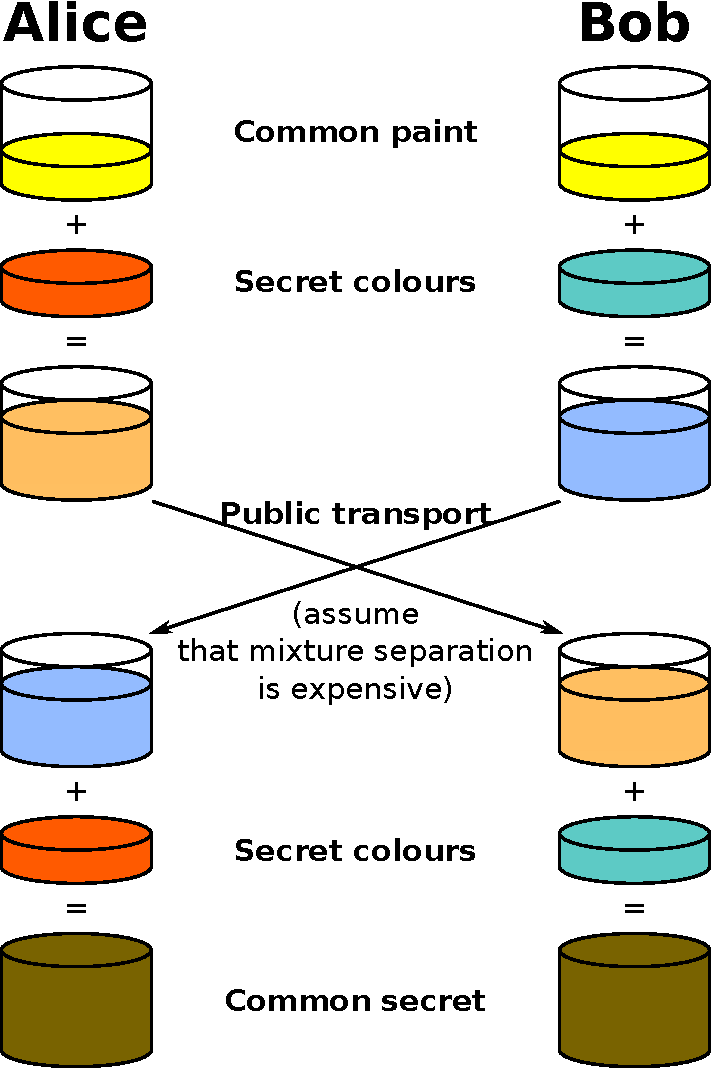
\includegraphics[scale=0.6]{./Figures/3-5-2a.pdf}
  \end{center}
  
  Unfortunately, however, we cannot easily turn graphics in to algorithms, and so we must define the formal process behind Diffie--Hellman\cite{Mao:2003uq}.
  
  \begin{enumerate}
    \item Given a large prime $p$ and $g$, an element in the finite field $F_p^*$,
    \item Alice picks an integer $a$ in $[1,p-1)$ and calculates $g_a = g^a \mod p$ and sends it to Bob.
    \item Bob picks an integer $b$ in $[1,p-1)$ and calculates $g_b = g^b \mod p$ and sends it to Alice.
    \item Alice and Bob computer $K = g_b^a$ and $K = g_a^b$, respectively.
  \end{enumerate}
  
  Given that the relationship $ab \equiv ba \mod (p-1)$ is valid, and the for Alice:
  
  \begin{center}
    $K = g^{ba} \mod p$
  \end{center}
  
  And for Bob:
  
  \begin{center}
    $K = g^{ab} \mod p$
  \end{center}
  
  We can see that both Alice and Bob's calculations will result in the same keying material.
  
  The secrecy of Diffie--Hellman is reliant on a problem known as the Computational Diffie--Hellman Problem. 
  
  \begin{mathdef}
    Given $g$, a generator element in the finite field $\mathbb{F}_q^*$, and ${g^a,g^b} \in F_q^*, 0 < a, b < q$, find $g^{ab}$.
  \end{mathdef}
  
  These values are available to an attacker, however they are not useful without being able to calculate $g^{ab}$ easily.
  
    \subsubsection{Implementation}
    
    In Java, two classes are necessary for a robust D--H implementation. Firstly, a key generator to create the public and private keys for both entitites.
    
     \lstinputlisting{../../sys/EnigmaApp/src/com/cyanoryx/uni/crypto/dh/KeyGenerator.java}
    
    Secondly, the actual algorithm implementation that, given a received public and local private key, will generate keying material as defined in RFC2631\footnote{\cite{Rescorla:1999aa}}.
    
    \lstinputlisting{../../sys/EnigmaApp/src/com/cyanoryx/uni/crypto/dh/KeyAgreement.java}
    
    Both \verb!KeyGenerator! and \verb!KeyAgreement! can be found in \emph{com.cyanoryx.uni.crypto.dh}.
    
    Using these implementations, a shared-key would be generated as so:
    
    \begin{enumerate}
      \item Alice generates a public and private key pair with \verb!KeyGenerator!, and sends the public half to Bob.
      \item Bob generates a key pair based on Alice's key using \verb!KeyGenerator!, and sends the public half to Alice.
      \item Both Alice and Bob use \verb!KeyAgreement! to generate keying material using both their private and public keys.
      \item Alice and Bob are now in possession of a shared session key that has not been sent between them, let alone in cleartext.
    \end{enumerate}
  
\section{Other Variations of Public-key Cryptography}

  \subsection{ElGamal}
  
  ElGamal differs from RSA and D--H in that it is not just a public-key encryption/decryption algorithm, but a public-key cryptosystem that is to be used not only to generate and share keys, but also encrypt the confidential messages to be sent using these keys. It utilises the one-way trapdoor function, and became popular due to the fact that it is based around the Computational Diffie--Hellman Problem and the Discrete Logarithm Problem, \cite{Mao:2003uq} \textsection pg.253, the latter of which is considered as an alternative to the integer factorisation problem.
  
  \paragraph{Key Generation and Sharing}
  
  Alice:
  
  \begin{enumerate}
    \item Chooses a random prime number $p$.
    \item As with D--H, calculates a multiplicative generator element $g$ in $\mathbb{F}_p^*$.
    \item Picks a random number $d$ where $d \in \mathbb{Z}_{p-1}$.
    \item Computes $e = g^x\mod p$.
    \item $d$ and $e$ are the private and public keys, respectively.
  \end{enumerate}
  
  \paragraph{Encryption}
  
  If Bob wishes to send a message $m$ to Alice,  he must:
  
  \begin{enumerate}
    \item Pick a random integer $k$ such that $k \in \mathbb{Z}_{p-1}$.
    \item Computer a pair of ciphertexts $(C_1,C_2)$ such that:
    \item $C_1 = g^k \mod p$
    \item $C_2 = e^km \mod p$
  \end{enumerate}
  
  And send the pair to Alice.
  
  \paragraph{Decryption}
  
  Upon receipt, Alice:
  
  \begin{enumerate}
    \item Calculates $m = C_1/C_2^d \mod p$.
  \end{enumerate}
  
  This can be proved by showing that:
  
  \begin{center}
    $C_1^d \equiv (g^k)^x \equiv (g^d)^k \equiv e^k \equiv C_2/(m \mod p)$
  \end{center}
  
    \subsubsection{Textbook Algorithm Insecurity}
    
    As we have said, textbook algorithms are defined as such because they are simply the core mathematical concept, with no additional security measures, and thus are very weak encryption schemes. The same stands for ElGamal -- it can leak parts of information. Commonly, a value $g$ (as defined above) is of order $r = $ord$_p(g) << p$ to improve efficiency\cite{Mao:2003uq} however if the message $m$ is not defined in the group $\langle g \rangle$ then a meet-in-the-middle attack -- for example, calculating the encrypted value of the plaintext for all possible keys and then decrypting for each key, which is likely to revel the correct keys -- can be made. 
    
    For a ciphertext $(C_1,C_2) = (g^k, e^km) \mod p$, an attacker Mallory can calculate $C_2^r \equiv m^r \mod p$. This is bad because it results in ElGamal no longer being a probabilistic encryption scheme, but a deterministic one. This means that a trial-and-error method of determining keys can take place, as above.
  
  \subsection{Rabin}
  
  The Rabin Public-Key Algorithm, created by Michael O. Rabin of Miller--Rabin fame, is a public-key cryptosystem that is based around the difficulty of calculating a square root, modulo a non-prime integer, which is equivalent to the difficulty of integer factorisation. It is a simple and efficient algorithm, and is implemented as so:
  
  \paragraph{Key Generation}
  
  Alice generates a key as in RSA:
  
  \begin{enumerate}
    \item Generate to large primes, $p$ and $q$.
    \item Compute the modulus $N = pq$.
    \item Pick a random integer $b$ such that $b \in \mathbb{Z}_N^*$.
    \item $(N,b)$ becomes the public key, while $(p,q)$ is the private key.
  \end{enumerate}
  
  \paragraph{Encryption}
  
  To encrypt a message $m$, Bob must:
  
  \begin{enumerate}
    \item Calculate ciphertext $c = m(m+b) \mod N$.
  \end{enumerate}
  
  \paragraph{Decryption}
  
  To decrypt a received ciphertext $c$, Alice must:
  
  \begin{enumerate}
    \item Solve the equation $m^2 + bm -c \equiv 0 \mod N$.
  \end{enumerate}
    
Due to its popularity, we will be using RSA as our main method of key exchange.

\section{Uses and going forward}

Now that we have formally defined the mathematics behind public-key cryptography and implemented them from prime number generation through to key generation and actual encipherment/decipherment, what can it be used for practically? 

In the context of our instant messaging application, could a secure public-key scheme like RSA be used to encrypt outgoing messages? Technically speaking, yes; however, practically, no primarily because of running time concerns: {\color{red}Add citation} public-key cryptography is significantly slower than using symmetric-key cryptography. The solution to this is to utilise both schemes such that they complement one another -- this is known as a digital envelope scheme.

\begin{center}
  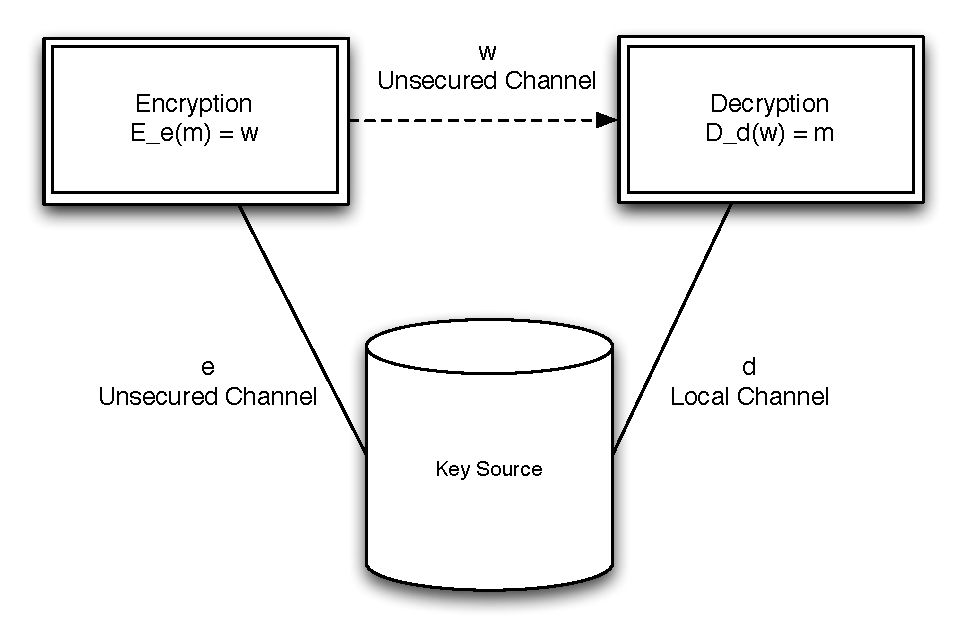
\includegraphics[scale=0.6]{./Figures/3-7a.pdf}
\end{center}

This is the standard process for sending an encrypted message $m$ via public-key cryptography. If instead we encrypt a session key for a symmetric algorithm, like AES, and send that securely then both entities will be in possession of a session key without it ever having been transferred in the clear.

\begin{center}
  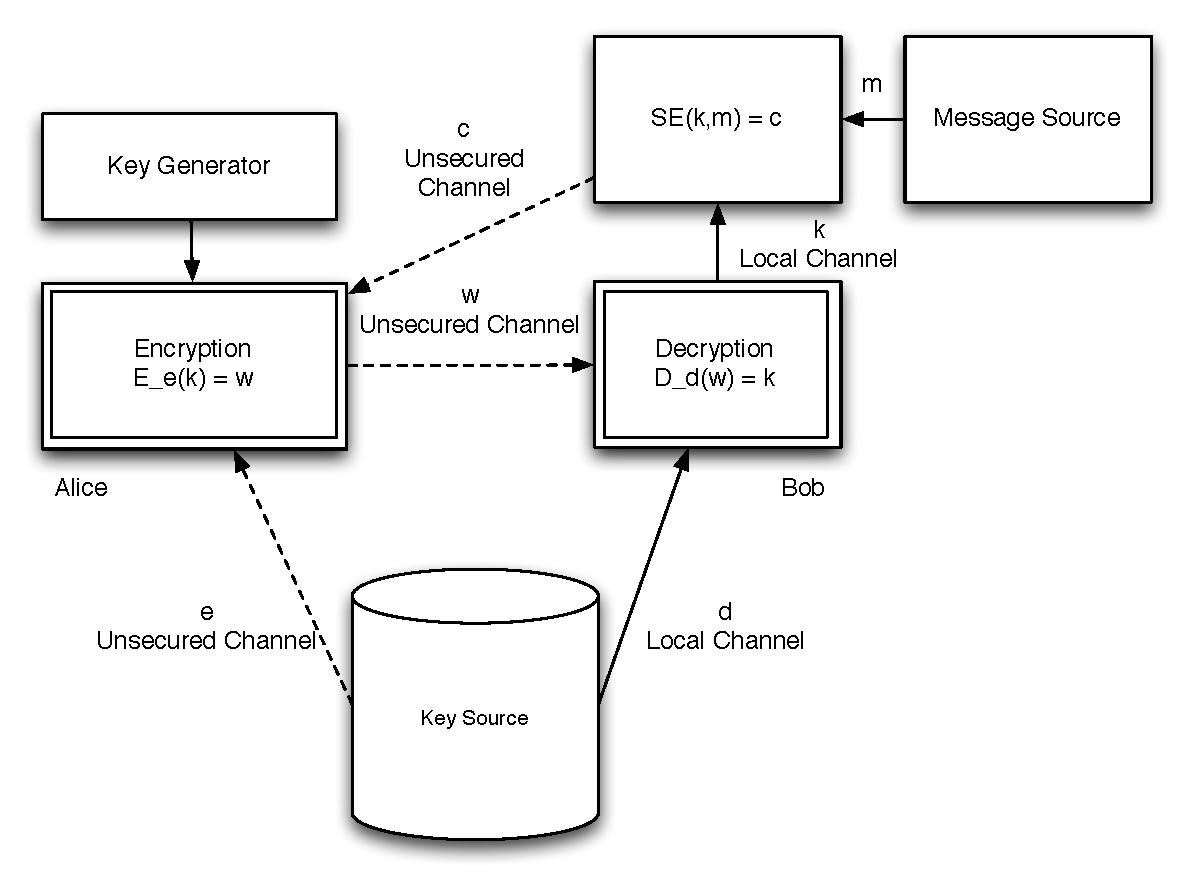
\includegraphics[scale=0.6]{./Figures/3-7b.pdf}
\end{center}

In this case, Alice generates and encrypts a key $k$ with Bob's public key and sends it to him, Bob then decrypts this and stores the key. Both Alice and Bob are now have the session key.

This is a simple and easy to implement solution using existing -- and open source -- technologies (without requiring any custom hardware) that we will be utilising as a key exchange mechanism in the Enigma application.

\subsection{Problems}

As considered in \emph{\textsection 2.4}, there is an issue with using public-key schemes for either message encryption or key encryption -- impersonation. The ideal public-key system should allow two entities to securely communicate by sharing their public keys without ever meeting to exchange session keys, however there is no "built-in" method for determining whether or not the public key you are using to encrypt a key is indeed the key of the entity with which you wish to talk to. 

\begin{center}
  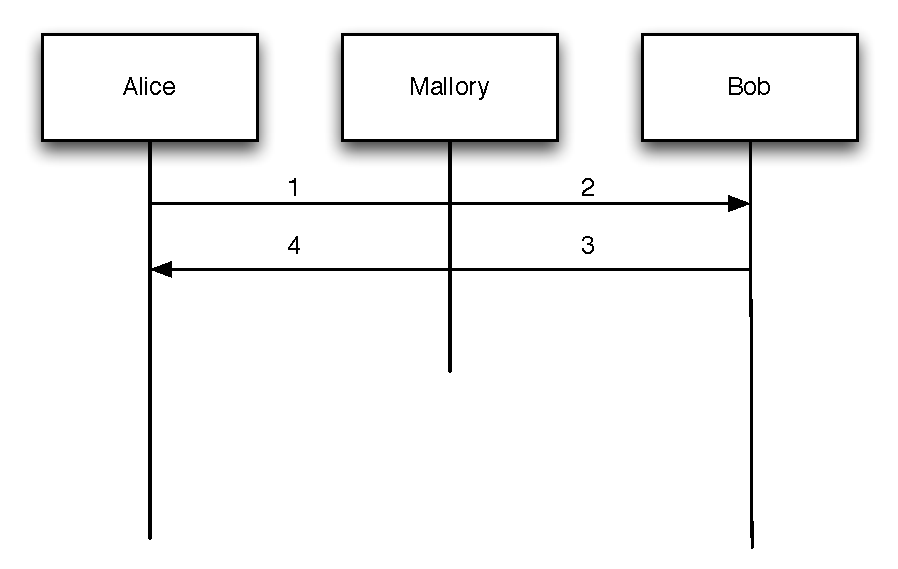
\includegraphics[scale=0.6]{./Figures/3-7-1.pdf}
\end{center}

\begin{enumerate}
  \item Alice sends her public key to who she thinks is Bob, however Mallory receives it.
  \item Mallory sends her own public key to Bob, masquerading as Alice.
  \item Bob encrypts a generated session key with Mallory's public key, and sends it to Mallory.
  \item Mallory decrypts the session key, and re-encrypts it with Alice's public key, and sends it to Alice.
\end{enumerate}

Here, Mallory is acting as a middle-man and unbeknownst to the other she gains access to the session key. Using this, she will be able to read and modify any messages sent between Alice and Bob, undetected.

\textsection 2.2 states that there are four requirements are necessary for a system to be considered secure:

\definecolor{gray}{RGB}{128,128,128}
\begin{enumerate}
	\item \textcolor{gray}{Confidentiality}
	\item \textbf{Authentication}
	\item \textcolor{gray}{Non-repudiation}
	\item \textcolor{gray}{Data Integrity}
\end{enumerate}

Here we are failing \textbf{authentication}. As we will see in Chapter 5, we can use another aspect of public-key cryptography -- digital signatures -- along with trusted third parties to identify and authenticate the entity with which we are communicating.

However, we are getting ahead of ourselves. The next step is to research and implement the symmetric ciphers that will be used to rapidly and securely encrypt the messages that will be transmitted between users. 

% Chapter 5

\chapter{Enigma: A Testbed} % Write in your own chapter title
\label{Chapter5}
\lhead{Chapter 5. \emph{Enigma: A Testbed}} % Write in your own chapter title to set the page header


\section{Description}
\section{Protocol}
\section{Interface} 

% Chapter 5

\chapter{Enigma: A Testbed} % Write in your own chapter title
\label{Chapter5}
\lhead{Chapter 5. \emph{Enigma: A Testbed}} % Write in your own chapter title to set the page header


\section{Description}
\section{Protocol}
\section{Interface} 

% Chapter 7

\chapter{Further Research} % Write in your own chapter title
\label{Chapter7}
\lhead{Chapter 7. \emph{Further Research}} % Write in your own chapter title to set the page header

???? 

% Chapter 7

\chapter{Further Research} % Write in your own chapter title
\label{Chapter7}
\lhead{Chapter 7. \emph{Further Research}} % Write in your own chapter title to set the page header

????

%% =====================
% APPENDICES

\addtocontents{toc}{\vspace{2em}} 

\appendix 

% Appendix A

\chapter{Enigma Application Software Requirements Specification}
\label{AppendixA}
\lhead{Appendix A. \emph{Enigma Application Specification}}

\section{Introduction}

\subsection{Purpose}

\subsection{Scope}



\subsection{Definitions}

\subsection{Overview}

\section{Overall Description}

\subsection{Product Perspective}

\subsection{Product Functions}

\subsection{User Characteristics}

\subsection{Constraints}

The software should \textbf{not} be considered for use in an environment where sensitive information is required to be shared which, if released, would pose a threat to life, cause injury to persons or damage to property, or any other result which could be considered damaging or illegal.

\subsection{Assumptions and dependencies}

% Appendix B

\chapter{Enigma Protocol Specification}
\label{AppendixB}
\lhead{Appendix B. \emph{Enigma Protocol Specification}}

\section{Introduction}

\section{Terminology}

\section{Definitions}

\section{Format}

\section{Commands}

\subsection{Connection}

A connection is represented by a streaming XML document, with the root element being \verb!<stream>!.

\begin{itemize}
	\item \textbf{Opening a connection:}
		\begin{verbatim}
			<stream  to="SERVER_NAME"
				         from="USER_NAME"
				         id="SESSION_ID"
				         return-port="LOCALHOST_INBOUND_PORT"
				         xmlns="enigma:client">
		\end{verbatim}
	\item \textbf{Closing a connection:}
		\begin{verbatim}
			</stream>
		\end{verbatim}
\end{itemize}

\subsection{Authentication}

\begin{itemize}
	\item \textbf{Toggling encryption:}
		\begin{verbatim}
			<auth stage="streaming"
			      id="SESSION_ID"
			      type="toggle">
			      [off|on]
			</auth>
		\end{verbatim} \\
		Note: this requires the agreement of both users. The connection should be closed if one user disagrees to change the current encryption status.
\end{itemize}

\begin{itemize}
	\item \textbf{Asserting the key agreement method:}
		\begin{verbatim}
			<auth stage="agreement"
			      id="SESSION_ID"
			      type="method">
			      [method type identifier]
			</auth>
		\end{verbatim} \\
\end{itemize}

\begin{itemize}
	\item \textbf{Publishing a certificate:}
		\begin{verbatim}
			<auth stage="agreement"
			      id="SESSION_ID"
			      type="cert">
			      [Base64 encoded Enigma Certificate]
			</auth>
		\end{verbatim} \\
\end{itemize}

\begin{itemize}
	\item \textbf{Publish an encrypted symmetric cipher key:}
		\begin{verbatim}
			<auth stage="agreement"
			      id="SESSION_ID"
			      type="key"
			      [method="CIPHER_ALGORITHM"]>
			      [Base64 encoded encrypted key]
			</auth>
		\end{verbatim} \\
\end{itemize}

\subsection{Messaging}

\begin{itemize}
	\item \textbf{Sending a message:}
		\begin{verbatim}
			<message  [to="REMOTE_USER_NAME"]
				          from="USER_NAME"
				          id="SESSION_ID"
				          [type=""]>
			    <body>MESSAGE_CONTENT</body>
			</message>
		\end{verbatim}
\end{itemize}

\subsection{Errors}

Errors do not have a specific element themselves, but are included as a subelement of any other tag, setting \verb!att:type! to \verb!error!.

\begin{itemize}
	\item \textbf{Sending an error:}
		\begin{verbatim}
			<element  [other attributes]
				          type="error">
			    <error type="ERROR_NUMBER">
			        ERROR_MESSAGE
			    </error>
			    [element contents]
			</element>
		\end{verbatim}
\end{itemize} 

\addtocontents{toc}{\vspace{2em}} 
\backmatter

%% =====================
% BIBLIOGRAPHY

\label{Bibliography}
\lhead{\emph{Bibliography}}  
\bibliographystyle{unsrtnat}  
\bibliography{Project}  % The references (bibliography) information are stored in the file named "Bibliography.bib"

\end{document}  % The End
%% ----------------------------------------------------------------